\chapter{Introduction}

\section{CubeSats}

CubeSats are nanosatellites with standardized cubic shape (as multiples of 10x10x10 cm\textsuperscript{3}) that are stored inside a standardized container during launch and deployed once the orbit is reached by the rocket upper stage. CubeSats are typically launched in bulks as secondary payloads and thus provide more affordable launch prices, plus more regular launch options and some flexibility in the launch opportunities.

In 1999 the CubeSat standard was created as a joint effort by professors Jordi Puig-Suari of California Polytechnic State University and Bob Twiggs of Stanford University \cite{heidt2000cubesat}. The standard specifies mainly the mechanical interface requirements of a 1 kg, 10x10x10 cm\textsuperscript{3} nanosatellite. Satellites adhering to this standard would be compatible with the Poly-PicoSatellite Orbital Deployer (P-POD), a standardized launch container developed as well at Stanford University \cite{nason2002development}. The P-POD is attached to the upper stage of a launch rocket, carries between one and three of such CubeSats and deploys them into orbit. As such, the P-POD provides a first degree decoupling of the interface between satellite and launch rocket and eases the launcher integration process significantly.

The motivation for the invention of the CubeSat standard was to enable graduate students to design, build, test and operate satellites within their academic curriculum. The first CubeSats were launched in June 2003 and led to an explosive growth of CubeSat launches in recent years. The success of CubeSats is attributed exactly to its standardized interface with respect to the launcher integration, which led to cheaper launch costs in the range of several tens of thousands of Euros and an accelerated launch preparation schedule.

Triggered by the success of CubeSats, a handful of start-up companies appeared during the second half of the first decade of 2000, and more followed. Founded mainly by graduates who worked on CubeSat missions during their studies, these companies kept strong ties with their (hosting) university, and focused mainly on supporting research and educational missions. Yet, despite having this academic background, the products were sold closed source, with some companies offering the design information for a significant surplus charge. Around the same time, industry and military entered the fast growing CubeSat sector and launched own CubeSat missions \cite{taraba2009boeing}. By 2013 a dramatic increase of CubeSats deployed in space is noticeable, as shown in Figure \ref{fig:CubeSats launched from 2003 to 2014}. Most of the recent CubeSats were launched as clusters or fleets under the flag of private companies. Nonetheless, the academic world takes the largest share among CubeSat developers, as shown in Figure \ref{fig:CubeSats that were launched from 2003 to 2014 grouped by ownership}. 

\begin{figure}[h]
\centering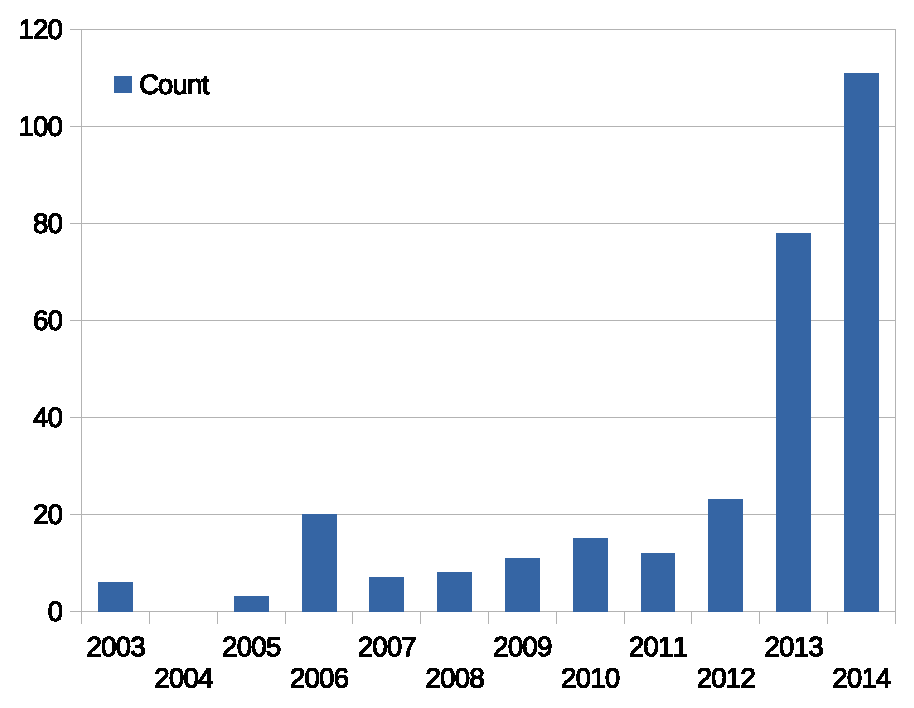
\includegraphics[width=0.6\linewidth]{fig/cubesats_launched_from_2003_to_2014}
\caption{CubeSats launched from 2003 to 2014. Compiled using data from M. Swartwout.}
\label{fig:CubeSats launched from 2003 to 2014}
\end{figure}

\begin{figure}[h]
\centering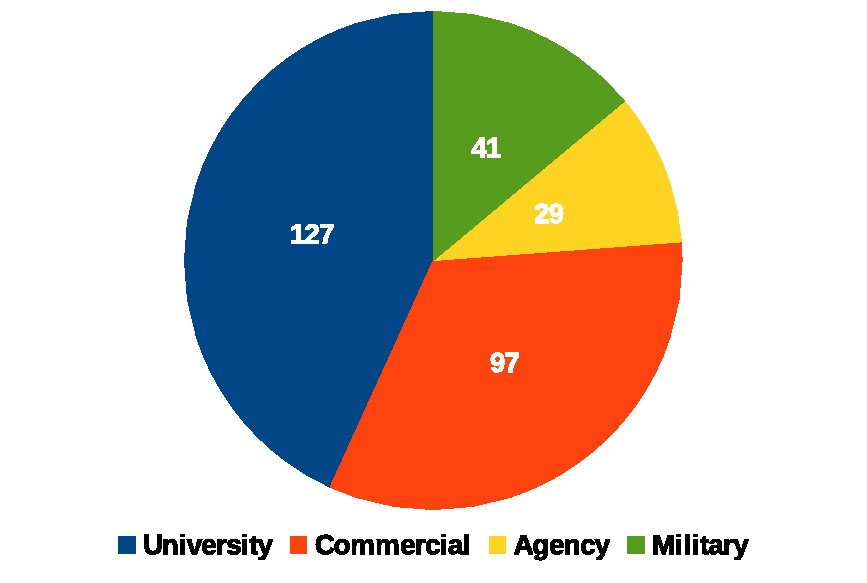
\includegraphics[width=0.8\linewidth]{fig/cubesats_launched_from_2003_to_2014_by_ownership}
\caption{Number of CubeSats that were launched from 2003 to 2014 grouped by ownership. Compiled using data from M. Swartwout.}
\label{fig:CubeSats that were launched from 2003 to 2014 grouped by ownership}
\end{figure}

From this it is evident that academia remains a major player in the CubeSat sector. As such, it has a strong impact on the future of the CubeSat program. CubeSats are an ideal tool for teaching hands-on space technology but they also offer a great chance for opening up the access to space technology to a much larger audience, including students and individuals from developing countries \cite{scholz2015toward}. 

\begin{comment}

\section{Open Source}

The current trend of increasing closed-source commercialization is counter-productive to the objective of opening the access to space. One side effect is that a number of universities have established ``centers of excellence'' for CubeSats, which capitalize on their in-house acquired knowledge. At the same time inter-university collaborations are minimal or not pursued at all. This is arguably not in the original interest of the CubeSat concept, which stipulates the free exchange of design information and lessons learned. 

Terrestrial open source software (OSS) is the backbone of modern society. It is present in almost every field of information technology, such as web servers, operating systems, software development tools, and mobile phones. Open source hardware (OSHW), as discussed in this context\footnote{Radio amateurs, hobbyists, and DIY communities have exchanged design information ever since; here we focus on projects that are made available to a wider public, mainly via the internet.}, is a relatively new phenomenon that follows the same principles: to allow anyone access to its sources for modification, sharing, building, and selling. 

\subsection{Definition}

The combination of open source software and open source hardware is referred to as \textbf{open design}. The recognized authorities for open source software regulation are the Free Software Foundation (FSF) and the Open Source Initiative (OSI), founded in 1985 and 1998, respectively. Both differ to some extent in their goals and values, but from a practical point of view agree on many aspects of what it means to produce free or open software. As a summary of the ten rules for open source definition, the OSI states \cite{opensource.org},

\textit{Open source software is software that can be freely used, changed, and shared (in modified or unmodified form) by anyone. Open source software is made by many people, and distributed under licenses that comply with the Open Source Definition.}

The definition of open source hardware is more complex. This stems from the fact that usage of hardware differs much from software and, being a relatively new phenomenon, less literature on that topic is available. See Lock \cite{lock2013open} for a thorough discussion on this subject. Also, software is easily copied and redistributed, which is not the case for hardware. Hardware modification and production requires access to drawings, schematics, diagrams, design rules, layouts, and other documents.  The Open Source Hardware Association (OSHWA) provides the following definition \cite{oshwa.org}:

\textit{Open source hardware is hardware whose design is made publicly available so that anyone can study, modify, distribute, make, and sell the design or hardware based on that design. The hardware's source, the design from which it is made, is available in the preferred format for making modifications to it.}

Broadly speaking, open source hardware is a physical artifact whose design information is made available under one of the legally binding recognized open source licenses.

\subsection{Intellectual Property Rights}

A number of mechanics are in place to protect the intellectual property of individuals and entities. The most relevant ones for open source design are discussed in the following.

\textbf{Copyright} grants the creator of original work the right to use and distribute it, and to define the conditions therefore. It is a legal concept that is protected well in most countries, and is usually in effect for a certain time, such as the lifetime of the author plus several decades. It applies to published and unpublished works. Main intention is to allow the author to benefit from their work, financially or else. Copyright is a very useful concept as it allows the author to decide on what to do with the work, such as to transfer it into the public domain.

Whereas copyright protects how information is presented, \textbf{patents} cover the subject matter of this information. For example, copyright law may restrict one from making copies of design files for a certain product, but it would not prevent one from making and using that product. Put differently, copyright only governs the expression of the idea, but not the idea itself. This is where patents come into play, which offer the right to exclude others from doing so. In short, patents ensure that the patent owner can take full ownership of its invention with the exclusion of others. Obviously, this is exactly the contrary of what open source design stands for.

\textbf{Trademarks} are typically names, slogans, or symbols, used for identification with goods or services. Trademark rights prevent others from using the same sign for their goods or services, but not from making or offering similar goods or services. As such, they provide a way to label offerings to make them recognizable and accredited by users \cite{anderson2010passport}.

\subsection{Open Source Licenses}

Creators of original work may either write license conditions on their own or adapt or modify existing licenses. Making use of existing licenses provides the advantage of a solid legal groundwork, and they are usually well understood and respected in the community. Basically, an open license is an agreement by the author(s) of original work to allow other people to make use of this work in accordance with the license regulations, without the need of paying licenses fees, as long as the terms of the license are followed. It grants rights to the product, that would otherwise be restricted through copyright or patent law.

Two main categories of open source copyright licenses exist: \textbf{strong copyleft} licenses that require that derivative work must be licensed under the same license; and \textbf{weak copyleft} (i.e. permissive) licenses, which permits the use of different license terms for derived works. The latter would allow modifiers to incorporate their open designs into closed proprietary designs or for merging them with projects which have adopted a different form of open license \cite{katz2012towards}.

Licenses for hardware and software differ naturally \cite{ackerman2008toward}. For software projects, the license ensures that the source code is made available. Hardware licenses on the other hand have to provide terms for the user rights on the design information as well as on the manufacturing and usage of the products. Various licenses are available for hardware and software projects and some of the major ones are briefly introduced in the following. See also \cite{webbink2010packaging} for an exhaustive treatment of open source licenses.

The \textbf{GNU General Public License (GPL)} and the \textbf{GNU Lesser General Public License (LGPL)} are published by the Free Software Foundation \cite{fsf.org}. The GPL allows the user to use, study, share, and modify the received software. It demands that these license conditions are also followed for copies of the original work or derived works. This constitutes a strong copyleft. The LGPL in contrast is a permissive free software license, similar to BSD license and MIT license, that allows developers and companies to use and integrate such work into their own (proprietary) software, without being required to apply the license conditions to their own work. The dominant usage of the LGPL is for software libraries.  

The \textbf{GNU Free Document License (FDL)} was designed for manuals, books, documentations, and other reference material, usually distributed together with open source hardware/software. Similar to the GPL, the FDL gives readers the rights to copy, distribute, and modify, requiring that all derivatives be licensed under the same terms (strong copyleft). A dedicated feature is that when copies are sold in larger quantities, the original document or source must be made available to the reader as well.

\textbf{Creative Commons (CC)} is a non-profit organization that has released several licenses \cite{creativecommons.org}. The creators of original work can easily choose a desired license ``a-la-carte'' that fits their needs in terms of which rights to be waived for others to make use of the work. CC licenses are used for all types of work that underlies copyright, including: books, plays, films, music, photographs, and websites. CC itself does not recommend the use of their licenses for software, although this has been done by some, such as for the Arduino boards.

The Tucson Amateur Packet Radio (TAPR) is an international amateur radio organization that published the \textbf{TAPR Open Hardware License (OHL)} in the flavor of a share-alike license that developers can apply to documentation and schematics \cite{tapr.org}. The key features of the license are that it firstly prevents the filing of patent infringements among people making use of OHL-licensed product, and secondly, that it requires modifiers to include both ``before'' and ``after'' versions of all files that were modified. The license is written in the form of a contract between author and recipient, and constitutes a strong copyleft.

The European Organization for Nuclear Research (Conseil europ\'{e}en pour la recherche nucl\'{e}aire, CERN) has issued the \textbf{CERN Open Hardware License (CERN OHL)} that, similar to what GPL is to software, defines the conditions to the use, copying, modification and distribution of hardware design documentation, and the manufacturing and distribution of products \cite{ayass2012cern}. As with other strong copyleft licenses, any modifications must be licensed under the same license conditions, in order to ensure that the whole community will continue benefiting from improvements.

\end{comment}

\section{Space Standards}

It is common practice to develop spacecraft based on unique designs which are specified and implemented on a project-by-project basis. Any reuse of these system design is usually a by-product of reuse of the whole spacecraft bus. While individual CubeSat developers may have established limited in-house standards or bespoken standards with vendors, these are generally closed and would require significant adaptation across other CubeSat missions.

Similarly, there exists little interface standardization for CubeSats which can be used by individual equipment and instrument developers. While it is true that there are a limited number of physical interfaces applicable for practical use in the space environment, the services and access to these interfaces vary considerably between implementations.

Within the CubeSat developer community there have so far been very few significant attempts to further standardize CubeSat missions. Apart from the CubeSat design specification \cite{cubesat_design_specification}, there exist only a few de-facto standards or best practices. Typically, the solutions that have been developed for CubeSat missions by individual developers are tied very much to the peculiarities of their CubeSat payload and mission objective, with little effort to create sustainable and reusable system components.

The result is that a multitude of CubeSat design solutions are in place, with each mission either inheriting past solutions or developing new ones. However, an increase in the number and complexity of missions and the cost of developing state-of-the-art high-speed data interfaces should trigger a re-thinking within the CubeSat community, towards application of a more standardized approach.

Standardization is an important tool to reduce risks, cost and improve both quality and communication between parties during the preparation and execution of space missions. This is true for any spacecraft mission, and CubeSats are no exception to it.

\subsubsection{Organizations}

A number of organizations exist that are concerned with the development of international standards applicable for space projects. As those standards are often based on vast experience from experts in the field, including lessons learned from past missions, they provide a valuable for meaningful standardization of almost any aspect of typical space missions. For most of these standards the particularities of the spacecraft are not important and hence can be applied to large satellite or CubeSats alike.

This book is concerned with the mapping of available international space standards to the various aspects of developing and running a CubeSat mission. The selection criteria for standards organizations were based on the following:

\begin{itemize}
\item Open: Standards shall be openly available to anybody, preferable through the internet.
\item Free: Standards shall be free of charge and fees.
\item International: Standards shall be written with international collaboration in mind.
\item Recent: Standards shall be implementable with state-of-the-art components.
\end{itemize}

The organizations found to comply well with these criteria are introduced briefly in the following sections.

The \textbf{Consultative Committee for Space Data Systems (CCSDS)} \cite{ccsds.org} was founded in 1982 for governmental and quasi-governmental space agencies to discuss and develop standards for space data and information systems. Currently composed of "eleven member agencies, twenty-eight observer agencies, and over 140 industrial associates," the CCSDS works to support collaboration and interoperability between member agencies through the establishment of data and system standards. The activities of the CCSDS are organized around six topic areas (see Figure \ref{fig:CCSDS Topic Areas}) and composed of many working groups.

The \textbf{European Cooperation for Space Standardization (ECSS)} \cite{ecss.nl} was initiated to harmonize the requirements from existing standards for space projects, and to provide a single, coherent set of standards for use in (but not limited to) all European space systems development and operation.

The goal of ECSS is to develop a common set of consistent standards for hardware, software, information and activities to be applied in space projects, so that life cycle cost are minimized, while continually improving the quality, functional integrity, reliability and compatibility of all elements of the project. It covers the disciplines shown in Figure \ref{fig:ECSS Disciplines}. 

\begin{figure}[h]
\centering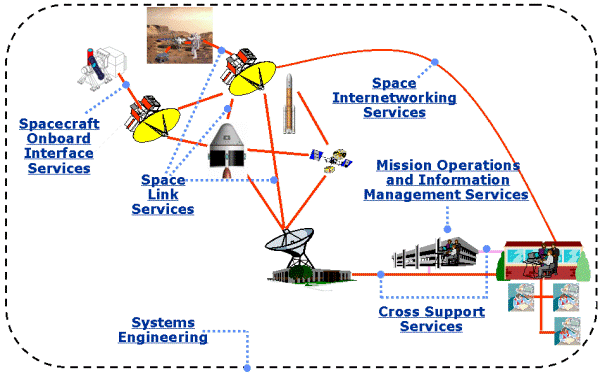
\includegraphics[scale=0.6]{fig/ccsds_topic_areas}
\caption{CCSDS Topic Areas}
\label{fig:CCSDS Topic Areas}
\end{figure}

\begin{figure}[h]
\centering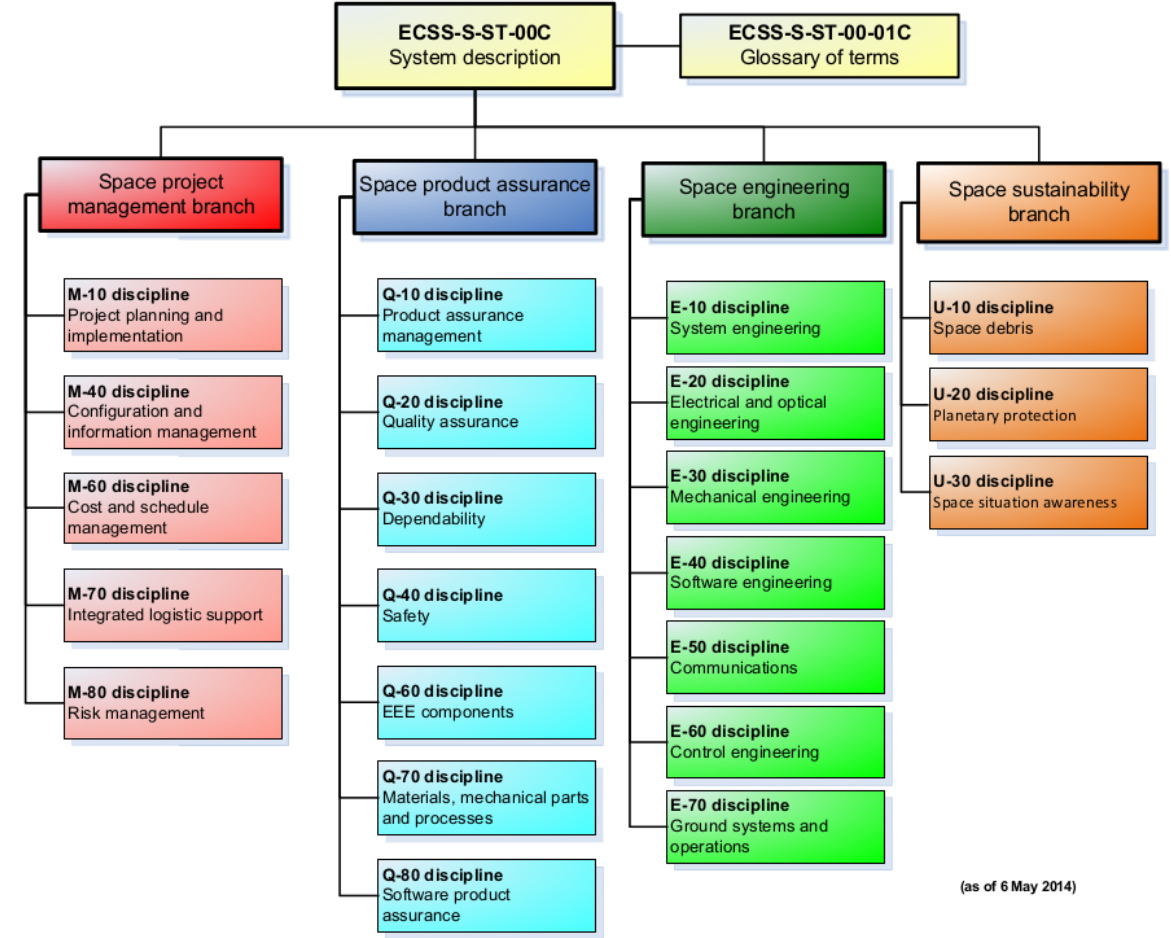
\includegraphics[scale=0.38]{fig/ecss_disciplines}
\caption{ECSS Disciplines}
\label{fig:ECSS Disciplines}
\end{figure}

The \textbf{Object Management Group (OMG)} \cite{omg.org} is an international, open membership, not-for-profit technology standards consortium. OMG Task Forces develop enterprise integration standards for a wide range of technologies and industries. including space industry. OMG modeling standards enable visual design, execution and maintenance of software and other processes. 

The \textbf{Organization for the Advancement of Structured Information Standards (OASIS)} \cite{oasis.org} is a global non-profit consortium that works on the development, convergence, and adoption of standards for security, energy, content technologies, emergency management, and other areas.
